%
% ---------------------------------------------------
%
% Trabajo Fin de Grado:
% Author: Víctor Hernández Pérez 
% Correo: alu0100697032@ull.edu.es
% Capítulo: Herramientas Software
%
% ----------------------------------------------------
%

\cleardoublepage
\chapter{Herramientas Software de desarrollo en Android} \label{chap:polytopes}  

En este capítulo se describen las herramientas software necesarias para la 
elaboración del TFG.

\section{Android Studio}

Android Studio \cite{URL::AndroidStudio} es un nuevo entorno de desarrollo 
integrado para el sistema operativo Android comercializado por Google, 
diseñado para ofrecer nuevas herramientas para el desarrollo de aplicaciones y 
alternativa al entorno Eclipse \cite{URL::Eclipse}, 
hasta ahora el IDE más utilizado.

¿Qué ofrece Android Studio? 
\begin{itemize}
\item Un entorno de desarrollo claro y robusto.
\item Facilidad para testear el funcionamiento en diversos tipos de dispositivos.
\item Asistentes y plantillas para los elementos comunes de programación en 
Android.
\item Un completo editor con muchas herramientas extra para agilizar el desarrollo 
de nuestras aplicaciones.
\end{itemize}

\subsection{Instalación}
Para instalar Android Studio es necesario disponer del Java Development Kit 
(JDK) \cite{URL::JDKInfo}. 

Una vez completada la instalación del JDK, se procede a la descarga del 
AndroidStudio \cite{URL::AndroidStudio}, del SDK de Android
\cite{URL::InstallSDK} y de todos los paquetes del SDK \cite{URL::SDKPackages} 
necesarios para asegurar la compatibilidad con los dispositivos Android en
los que se desee desarrollar.

\subsection{Primeros pasos en Android Studio}

Antes de comenzar con el desarrollo de la aplicación propuesta para el TFG, se 
realizaron una serie de tutoriales \cite{URL::GettingStarted, URL::SavingData} 
para familiarizarse con el uso de AndroidStudio así como de todo el entorno Android.

\section{Jasig}

Jasig \cite{URL::Jasig} es un Servicio de Autenticación Centralizada, Central 
Authentication Service (CAS \cite{URL::CAS}) en inglés.  
Está orientado a aplicaciones web y soporta multitud de protocolos de comunicación 
entre el servidor y el cliente así como: 
CAS, SAML, Oauth \cite{URL::Oauth} y OpenID \cite{URL::OpenID}.

\section{Django Allauth}

Django Allauth \cite{URL::allauth} es una aplicación en Django \cite{URL::Django} 
que permite autenticación local (usuario/contraseña) y autenticación social 
(Facebook, Twitter y muchos otros más). La instalación se hace mediante el 
sistema de gestión de paquetes de Python \cite{URL::Python} (pip), 
una vez instalado se ha de configurar apropiadamente el fichero settings de la 
aplicación Django e indicar qué proveedores (para la autenticación social) son 
necesarios. Y por último configurar las urls y migrar las bases de datos. Una vez 
hecho todo lo anterior el servidor estálisto para porder ser arrancado.

\section{Comunicación aplicación Android y el servidor}
La idea de la autenticación social es la siguiente y su unión con el servidor es 
la siguiente. Supongamos Facebook como proveedor de autenticación. En la aplicación 
móvil el usuario se autentica a través de Facebook el cual devuelve un Access Token
si resulta satisfactorio el proceso. En el caso de las aplicaciones móviles se trata 
de un token de larga duración (60 días de duración). Este token o identificador 
se actualiza una vez al día si el usuario hace una solicitud a los servidores de 
Facebook. Si el identificador llegará a caducar el usuario deberá repetir el proceso
de autenticación. Este token es enviado a nuestro servidor el cual comprueba su validez
a través de una petición a Facebook, en caso de que sea válido el usuario es considerado
autenticado en nuestro servidor y se utilizará dicho token para poder acceder a los 
distintos servicios disponibles.

\section{AppTui}

La aplicación del Observatorio appTUI \cite{URL::appTUI} es una aplicación gratuita para smartphones 
que tiene como finalidad ayudar a los usuarios de la TUI a sacar el mayor partido de 
todas las ventajas y servicios de su tarjeta. 

La TUI se vincula a la aplicación mediante la lectura de un código QR asociado a cada tarjeta. 
A partir de ese momento el usuairo puede, de forma sencilla, cómoda y segura, acceder a la 
información de todos los servicios TUI de su universidad, con la ventaja de poder recibir además
todas las alertas recordando reservas realizadas, así como las novedades y, en general, toda 
la información necesaria para hacer más ágil la gestión académica y administrativa dentro de la Universidad.

\begin{figure}[h]
	\centering
	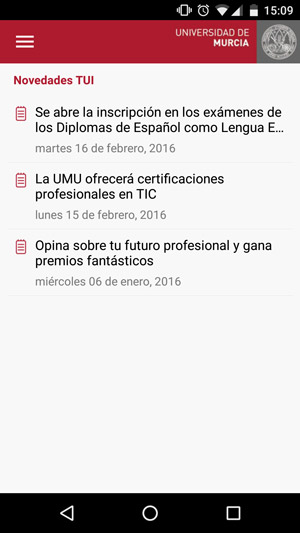
\includegraphics[width=0.3\columnwidth]{news.png}
	\caption{Vista de noticias de appTUI}
	\label{fig:ejemplo}
\end{figure}

Se ha seguido algún estilo similar para \App{} ...

\begin{figure}[h]
	\centering
	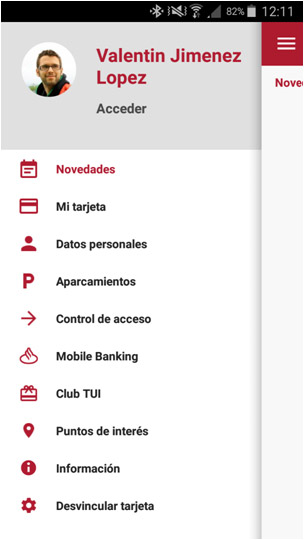
\includegraphics[width=0.3\columnwidth]{nav_view.png}
	\caption{Vista de navegación de appTUI}
	\label{fig:ejemplo}
\end{figure}

\subsection{Instalación}
...


